% Copyright (C) 2015 XPARCH, Ltd. <info@xparch.com> 

\documentclass{hitec}
\title{Simulating \textsc{Parallela} \textsc{P160X} boards in
  \textsc{Prazor} simulator}
\author{David Greaves and Milo\v{s} Puzovi\'c}
\confidential{}
\usepackage{graphicx}
\usepackage[colorlinks]{hyperref}
\usepackage{color}
\usepackage{pifont}
\usepackage{multirow}
\usepackage{wasysym}

\setlength{\marginparwidth}{1.2in}
\let\oldmarginpar\marginpar
\renewcommand\marginpar[1]{\-\oldmarginpar[\raggedleft #1]%
{\raggedright #1}}    

\newenvironment{checklist}{%
  \begin{list}{}{}% whatever you want the list to be
  \let\olditem\item
  \renewcommand\item{\olditem -- \marginpar{$\Box$} }
  \newcommand\checkeditem{\olditem -- \marginpar{$\CheckedBox$} }
}{%
  \end{list}
}   

\begin{document}
\maketitle
\tableofcontents
\section{Introduction}
This document describes design decisions that were made in order to
simulate the \textsc{Parallela} board in the \textsc{Prazor}
simulator~\cite{parallela}. The \textsc{Parallela} board is a high performance
computing platform based on a dual-core \textsc{ARM-A9 Zynq}
System-On-Chip and \textsc{Adapteva}'s \textsc{Epiphany} multicore
coprocessor. There are three different commercially available models
that are targeted to \textit{microserver}, \textit{desktop} and
\textit{embedded} markets. The main differentiator between these
models is the host processor and FPGA logic. The host processor in
microserver and desktop model is \textsc{Xilinx Zynq} dual-core
\textsc{ARM A9 XC7Z010}, while on embedded model the host processor is
\textsc{Xilinx Zynq} dual-core \textsc{ARM A9 XC7Z020}. The only
difference between these two host processor is clock rate and size of
caches and since these characteristics are parametirised in the
\textsc{Prazor} simulator we are able to simulate both processors. The
difference in FPGA logic is in number of \textit{logic cells} and
\textit{DSP slices}. The microserver and desktop models have 28K logic
cells and 80 DSP slices, while the embedded model has 80K logic cells
and 220 DSP slices. Since at the moment we are not simulating FPGA
logic in \textsc{Prazor} this difference is of no concerns to us. 

The rest of the document is organised as follows. In
Section~\ref{sec:implementation} we describe in details
\textsc{SystemC} modules that are used to simulate various parts of
the \textsc{Parallela} board. Section~\ref{sec:evaluation} discusses
techniques that will be used to evaluate performance and power usage
reported by the \textsc{Prazor} simulator versus numbers reported by
running the same benchmarks directly on the \textsc{Parallela} board. 
\section{Implementation}
Figure~\ref{fig:parallela} shows \textsc{SystemC} modules that were
used to simulate the \textsc{Parallela} board. From this Figure it is
possible to separate implementation of simulation of
\textsc{Parallela} board into five parts: host \textsc{ARMv7-A} CPU core
model (Section~\ref{ref:host}), memory management unit (TLB and page table, L1 and L2 caches and snoop control
unit, Section~\ref{ref:mmu}), DRAM controller and simulator
(Section~\ref{ref:dram}), \textsc{Epiphany} coprocessor (Section~\ref{ref:epiphany}), 
and toolchain (Section~\ref{ref:toolchain}) to be used to compile application to machine code
runnable by the host processor. 

\begin{figure}
\begin{center}
\includegraphics[width=0.97\textwidth,keepaspectratio=true]{parallela.pdf}
\end{center}
\caption{\textsc{SystemC} modules used to simulate \textsc{Parallela} board.}
\label{fig:parallela}
\end{figure}

There is one important assumption that we make in the \textsc{SystemC}
model presented in Figure~\ref{fig:parallela} about the
\textit{connection} between the host processor and \textsc{Epiphany}
coprocessor. When one of the nodes in the mesh network of
\textsc{Epiphany} coprocessor requests access to the memory that is
off-chip (i.e. DRAM) then requests will be sent along
\textsc{Epiphany}'s east \textsc{eLink} to the FPGA. It is important to
note that by design of \textsc{Parallela} board anything sent to the
west \textsc{eLink} will simply disappear, while south and north
\textsc{eLinks} are used for the expansion boards. Once the off-chip
memory request has been received by the FPGA the address in the memory
request will be translated from the \textsc{Epiphany}'s address space
(from \texttt{0x8e000000} to \texttt{0x8fffffff}) to the physical
address space (from \texttt{0x1e000000} to \texttt{0x1fffffff}) and
forwarded to the host processor. The host processor is aware that that
region of the physical address space is reserved for the communication
with the \textsc{Epiphany} coprocessor and can be only accessed for
that purpose. In our simulation address translation that is performed on
\textsc{Parallela} board is modelled inside the mesh node that is in
the top-left corner of the \textsc{Epiphany}'s mesh network. We
believe this model to be accurate enough and it does not require
modelling of the FPGA logic. 

The rest of this Section describes implementation details of each of
five parts of simulator introduced previously. 

\subsection{Host processor}
\label{ref:host}
The \textsc{Xilinx Zynq} programmable System-on-Chip contains
dual-core \textsc{ARM Cortex-A9} based application
processor unit with \textsc{ARMv7-A} architecture. This CPU can do up to 2.5DMIPS/MHz and has frequency
up to 1 GHz. On \textsc{Parallela} board this CPU is clocked at
800MHz. Furthermore. The Cortex-A9 architecture was designed to be highly-efficient,
dynamic length, multi-issue superscalar, out-of-order
microarchitecture with 8-stage pipeline~\cite{cortexa9}. 

The pipeline supports up to \textit{\underline{four} instruction cache line prefetch-pending} and
between \textit{\underline{two} and \underline{four} instructions per cycle forwarded continuously
into instruction decode}. The instruction decode stage is capable of
\textit{decoding \underline{two} full instructions per cycle}. It supports \textit{speculative
execution} of instructions, \textit{increased pipeline utilisation} by
removing data dependencies between adjacent instructions,
\textit{\underline{four} data cache line fill requests} and
\textit{out of order write back of instructions}. 

Based on the current status of \textsc{Prazor} simulator the following
new features need to be implemented in order to be able to simulate
the host processor found on \textsc{Parallela} board and described in
the previous paragraphs:

\begin{checklist}
\item Full support of \textsc{ARMv7} microarchitecture instruction set -
  \textbf{Must Have}
\item Full support of \textsc{ARM Thumb-2} instruction set -
  \textbf{Must Have}
\checkeditem Full support of \textsc{ARM NEON} media-processing
instruction set - \textbf{Nice To Have}
\end{checklist}

\subsection{Memory management unit (MMU)}
\label{ref:mmu}
\subsubsection{TLB and page table}
In order to be able to compare \textsc{Prazor} to the other simulators
it would be ideal if we could run \textsc{Linux} operating system on
it. The main missing part in the current implementation is that
\textit{translation lookaside buffer} (TLB) and \textit{page table} walking algorithm were not
implemented. As a part of this work we are going two implement TLB and
page table walking. It is important to notice that TLB and page table
walking can be implemented as pluggable \textsc{SystemC} module (as
illustrated by block \textsc{MMU} in Figure~\ref{fig:parallela}) or it
can be part of \textsc{ARM} core (\textit{composite reuse
  principle}). We will provide both implementation where
\textsc{SystemC} module will be a wrapper around concrete
implementation of TLB and page table walking algorithm. 

Thus, the following work needs to be done:

\begin{checklist}
\item Implement coprocessor 15 form ARMv7 microarchitecture because
  registers present in that coprocessor are needed in order to make
  translation lookaside buffer and page table walking algorithm work -
  \textbf{Must Have}
\item Implement translation lookaside buffer - \textbf{Must Have}
\item Implement page table walking algorithm - \textbf{Must Have}
\checkeditem Implement \textsc{SystemC} wrapper around the
implementation of translation lookaside buffer and page table walking
algorithm so that this unit can be made pluggable - \textbf{Nice To Have}
\end{checklist}

\subsubsection{Caches}
The current implementation of the memory management unit in the
\textsc{Prazor} simulator consists of standard snooping-based MESI
coherent protocol and advanced \textit{hammer} MOESI cache protocol
that is found on the most modern \textsc{AMD Opteron} processors. One
of the main problems behind the current implementation of MMU is the
lack of generality between these two different implementation as there
is a lot of conditional code that is executed depending on the
coherence protocol used. We are planning to remove this limitation by
implementing \textsc{ACE} (\textsc{AXI} Coherence Extensions) protocol
specification. This specification can implement various different
policies such as directory based, snoop filter or no snoop filter and
various different coherence protocols such as MSI, MESI and
MOESI. Table~\ref{tab:acestates} shows five states in which cache line
can be, while Table~\ref{tab:acemap} shows the mapping between ACE and
MOESI cache line states. 

\begin{table}
\begin{center}
\begin{tabular}{r|c|c|c|}
\multicolumn{1}{c}{} & \multicolumn{2}{c}{\textbf{Valid}} & \multicolumn{1}{c}{\textbf{Invalid}} \\
\multicolumn{1}{c}{} & \multicolumn{1}{c}{\textbf{Unique}} & \multicolumn{1}{c}{\textbf{Shared}} & \multicolumn{1}{c}{} \\
\cline{2-4}
\textbf{Dirty} & Unique Dirty & Shared Dirty & \multirow{2}{*}{Invalid} \\
\cline{2-3}
\textbf{Clean} & Unique Clean & Shared Clean &  \\
\cline{2-4}
\end{tabular}
\caption{\textsc{ACE} cache line states}
\label{tab:acestates}
\end{center}
\end{table}

\begin{table}
\begin{center}
\begin{tabular}{c|c|c}
\textbf{ACE} & \textbf{MOESI} & \textbf{ACE meaning} \\
\hline
UniqueDirty & Modified (M) & Not shared, dirty, must be written back \\
SharedDirty & Owned (O) & Shared, dirty, must be written back \\
UniqueClean & Exclusive (E) & Not shared, clean \\
SharedClean & Shared (S) & Shared, clean or dirty, no need to write back \\
Invalid & Invalid (I) & Invalid \\
\end{tabular}
\caption{Mapping between \textsc{ACE} and MOESI cache line states}
\label{tab:acemap}
\end{center}
\end{table}

The cache line changes state once it receives one of the transactions
shown in Figure~\ref{fig:acetrans}. For the brevity we only illustrate how
memory request sent from the \textsc{Epiphany} coprocessor is
satisfied by the host processor that has the requested memory address
in L1 cache. For the full description of each transaction please refer
to the official documentation~\cite{acedoc, acedoc2} about the
\textsc{ACE} protocol. 

\begin{figure}
\begin{center}
\includegraphics[width=0.97\textwidth,keepaspectratio=true]{acetransactions.pdf}
\end{center}
\caption{Transactions supported by the \textsc{ACE} protocol.}
\label{fig:acetrans}
\end{figure}

Figure~\ref{fig:aceexec} shows what happens in the \textsc{ACE} protocol if
\textsc{Epiphany} coprocessor wants to write to a cache line that is in
\textit{UniqueDirty} state in L1 cache of the second core in the host
processor. First, the \textsc{Epiphany} coprocessor will send request to the
cache controller (in this case snoop control unit) that it wants to write to
address \texttt{A}. Type of this request is going to be \textit{WriteUnique}
because \textsc{Epiphany} coprocessor is not cached. Once snoop control unit
(SCU) receives this request it will send to all coherent caches
\textit{CleanShared} transaction. This transaction will find that cache line in L1
cache of the second core is in \textit{UniqueDirty} state and that it should be
written back to the secondary storage. As a result of this the cache will send
\textit{WriteBack} transaction with data to the SCU that will be then forwarded
to the secondary storage. Once this transaction has completed the SCU you will
inform Epiphany coprocessor that it can now write to address \texttt{A}.

\begin{figure}
\begin{center}
\includegraphics[width=0.97\textwidth,keepaspectratio=true]{aceexec.pdf}
\end{center}
\caption{Execution scenario of a \textit{WriteUnique} transaction.}
\label{fig:aceexec}
\end{figure}

Another problem with the current implementation of the MMU is that we cannot
guarantee that all methods are \textit{reentrant} and \textit{thread-safe}. The
main stumbling block is the implementation of the coherence checks where the
cache that is checking for the line simply invokes method to check for the same
line in the caches that are in the same coherence groups. This can lead to
inconsistent states for the cache lines if caches that are being checked are
operating on parts of that cache line (for example, when we have \textit{false
  sharing}). To overcome this problem instead of using \textit{cache coherence
  groups} we will replace them with the \textit{Snoop Control Unit} and keep
caches consistent using the \textsc{ACE} protocol. This will also enable us to
remove locks that we have at the moment that make access to the caches
sequential. 

Therefore, the following works needs to be done for the memory management unit:
\begin{checklist}
\item Record metrics for certain set of benchmarks that collect how many times
  each lock has been taken and proportion of cache lines that has been accessed
  simultaneously by caches in the same coherent group. Use this data to discuss
  how contention can be modelled at the end of simulation - \textbf{Must have},
\item Implement \textsc{ACE} protocol and replace the current cache lines states
  transition diagram with it - \textbf{Must have},
\item Replace cache consistent groups with Snoop Control Unit - \textbf{Must
  have},
\item Run the new implementation in \textsc{SystemC} multi-core simulator -
  \textbf{Must have}. 
\end{checklist}

The following list is a list of features that are \textbf{nice to have} and are closely
related to the characteristics of \textsc{ARM Cortex A9}
microarchitecture. Since most of these features are switched off by default we
do not consider them as the main necessity for simulating \textsc{Parallela}
board in \textsc{Prazor} simulator:
\begin{checklist}
\checkeditem \textbf{Speculative read} - at the same time when request is send
to L1 cache it is also sent to L2 cache in order to reduce potential latency,
\checkeditem \textbf{Data and instruction prefetching} - there is a possibility
to automatically prefetch both data and instructions from the caches from the
cache line that is immediately next to the one that was requested,
\checkeditem \textbf{Clock gating} - L2 cache controller can automatically stop
clock when no requests has been received after a few cycles. The clock is
reactivated as soon as new request arrives,
\checkeditem \textbf{L2 power modes} - L2 cache has four different modes:
\textit{run}, \textit{standby}, \textit{dormant} and \textit{shutdown}. 
\checkeditem \textbf{Small loop optimisations} - there is a \textit{small loop
  memory} coupled to the instruction cache that is used to store small loops
that are less then 64 bytes of instructions. 
\end{checklist}

\subsection{DRAM controller and simulator}
\label{ref:dram}
The \textsc{Parallela} board uses 1GB 32-bit wide DDR3L SDRAM for off-chip
memory. In order to simulate this memory we will be using \textsc{SystemC}
module that wraps a cycle accurate memory system simulator
\textsc{DRAMSim2}~\cite{dramsim2}. No changes are needed to the current
implementation of the \textsc{SystemC} wrapper in order to simulate
\textsc{Parallela} board in the \textsc{Prazor} simulator. 

\subsection{\textsc{Epiphany} coprocessor}
\label{ref:epiphany}
The \textsc{Epiphany} coprocessor is a multicore, scalable, shared memory,
parallel computing fabric~\cite{epiphany}. It can contain 16 or 64 \textit{computing
nodes} that are arranged in two-dimensional array. These computing nodes are
connected by a low-latency mesh network-on-chip. Figure~\ref{fig:epiphany} shows
the implementation of the \textsc{Epiphany} architecture in \textsc{SystemC}
with a computing node zoomed in. 

\begin{figure}
\begin{center}
\includegraphics[width=0.97\textwidth,keepaspectratio=true]{epiphany.pdf}
\end{center}
\caption{Implementation of the \textsc{Epiphany} architecture in \textsc{SystemC}}
\label{fig:epiphany}
\end{figure}

Each computing node contains a \textit{\underline{superscalar}},
\textit{\underline{floating-point}}~\textsc{RISC} CPU. This CPU can execute
\textit{\underline{two}} floating-point operations and a 64-bit memory load
instruction on every clock cycle. The computing node has a local memory that
supports simultaneous instruction fetching, data fetching and multicore
communication. To achieve this, the local memory is divided int for 8-byte-wide
banks each 8KB in size, giving in total 32KB of local memory. 

The CPU core and memories are connected to a \textit{mesh-node crossbar
  switch}. The crossbar implements fixed-priority arbitration and it is only
needed when there is a potential for a shared-resource conflict. The access
priorities needed to resolve conflicts are listed in the official
documentation~\cite{epiphany}. 

The connections between different computing nodes are managed by \textit{network
interface} and \textit{router}. There are three different types of transaction
traffic. The first type is \textit{rMesh} and this is used for sending read
requests with throughput of 1 read transaction every 8 clock cycles in each
routing direction. The second type is \textit{cMesh} and this is used for write
transaction destined for on-chip mesh node with throughput of 8
bytes/cycle. Latency of write transactions is $1.5$ clock cycles per routing hop. The
final type is \textit{xMesh} that is used for write transactions to off-chip
memory. In the implementation proposed in this document the top-right computing
node with coordinates $(32,15)$ in Figure~\ref{fig:epiphany} is connected to
off-chip memory and only that computing node is responsible for sending data
off-chip. This is achieved by compiler from the toolchain that compiles code
such that all off-chip access is encoded in address by setting first 6 upper bits to
be $32$ and second 6 upper bits to be in the range from $32$ to $63$. The full
details behind the routing protocol and arbitration schemes can be found in the
documentation on \textsc{Epiphany}~\cite{epiphany}. 

Therefore, to implement \textsc{Epiphany} architecture in the \textsc{Prazor}
simulator the following steps must be taken:

\begin{checklist}
\item Implement \textsc{RISC} CPU core with \textsc{Epiphany} instruction set
  architecture described in Appendix in~\cite{epiphany} - \textbf{Must have}
\item For local memories use the existing implementation of \texttt{smallram}
  but add support for transactional access - \textbf{Must have}
\item Implement crossbar switch with arbitration as described in~\cite{epiphany}
  - \textbf{Must have}
\item Implement network interface and router with routing protocol and
  arbitration as described in~\cite{epiphany} - \textbf{Must have}
\item Parametirised the connections between computing nodes such that mesh
  networks with a different number of computing nodes can be created easily -
  \textbf{Must have}
\end{checklist}

\subsection{Toolchain}
\label{ref:toolchain}
There are two different toolchains to consider: \textsc{GCC} and
\textsc{LLVM}. Recently \textsc{LLVM} toolchain has been receiving a lot of
attention because of its modular design and ease of extension. Although there exists a pass
in the \textsc{LLVM} framework that can compile code for \textsc{ARMv7}
instruction set architecture there are no passes that can target
\textsc{Epiphany} instruction set architecture. Some work has been started a
year ago to add back end pass to the \textsc{LLVM} framework but it has been
dropped. The code is still available on \texttt{github}~\cite{llvmepiphany} and we can pick it up if
there is a need to use \textsc{LLVM} framework. 

As a result of lack of support
for \textsc{Epiphany} instruction set architecture in the \textsc{LLVM}
framework the toolchain used in this project will be used is \textsc{GCC}. 

\label{sec:implementation}
\section{Evaluation}
\label{sec:evaluation}
The main goal of this project is to compare the accuracy of the
\textsc{Prazor} simulator against a real hardware platform: \textsc{Parallela}
board. As far as we are aware the most recent and the only work that has similar
goal to ours is presented in~\cite{eval}. In that work the authors investigated the
sources of error in \textsc{gem5}~\cite{gem5} by validating it against the \textsc{ARM}
Versatile Express TC2 development board. After making some modifications to
the simulator they were able to achieve a mean percentage runtime error of
$5\%$ and a mean absolute percentage runtime error of $13\%$ for the \textsc{SPEC}
CPU2006 benchmarks and mean percentage runtime error of $-11\%$ and $-12\%$
for a single and dual-core runs respectively and mean absolute percentage
runtime error of $16\%$ and $17\%$ for a single and dual-core runs
respectively for the \textsc{PARSEC} benchmarks. Furthermore, authors
in~\cite{eval} have investigated accuracy of several microarchitectural
statistics and showed that they were able to achieve accuracy within $20\%$
on average for a majority of them. They have concluded that main source of the
errors was modelling of similar, but not identical components. 

In order to achieve our goals and based on the results obtained in~\cite{eval}
we are planning to do the following:
\begin{checklist}
\item Collect runtime and scaling accuracy for \textsc{PARSEC} benchmarks. This
  metrics will be used to evaluate the whole simulator shown in Figure~\ref{fig:parallela} -
  \textbf{Must have},
\item Collect observed memory access latency and bandwidth measurements for
  \textsc{PARSEC} benchmarks. This
  metrics will be used to evaluate memory management unit and DRAMSim2 of
  \textsc{PRAZOR} simulator - \textbf{Must have},
\item Collect cache miss and access stats for \textsc{PARSEC} benchmarks. This
  metric will be used to evaluate memory management unit only - \textbf{Must have}
\item Collect branch and TLB miss states for \textsc{PARSEC} benchmarks. This
  metric will be used to evaluate behaviour of simulated \textsc{ARM} core. 
\item Collect power and energy consumption for \textsc{PARSEC} benchmarks. This
  metric will be used to evaluate \textsc{TLM Power3} library - \textbf{Must
    have}. 
\end{checklist}

We are planning for the simulation of \textsc{Parallela} board in the
\textsc{Prazor} simulator to achieve the following accuracy:
\begin{checklist}
\item Mean percentage runtime error between $7\%$ and $10\%$ for a single and dual-core
  runs of the \textsc{PARSEC} benchmarks,
\item Mean absolute percentage runtime error within $10\%$ for a single and
  dual-core runs of the \textsc{PARSEC} benchmarks,
\item Accuracy of microarchitectural statistics between $10\%$ and $15\%$ for
  the \textsc{PARSEC} benchmarks and
\item Mean percentage power and energy consumption within $10\%$ for a single
  and dual-core runs of the \textsc{PARSEC} benchmarks.
\item Mean absolute percentage power and energy consumption within $15\%$ for a
  single and dual-core runs of the \textsc{PARSEC} benchmarks. 
\end{checklist}

Finally, since we are planning to put every physical/logical hardware
unit that we are modelling in \textsc{Prazor} in a separate thread we
should be able to see decrease in simulation time as number of cores
dedicated for the simulator is increased. Therefore, we plan to do the
following:

\begin{checklist}
\item Check to see if \textsc{SystemC} kernel can run in multicore
  mode. If not investigate how difficult would it be to modify it such
  that it can run in multicore mode - \textbf{Must Have}.
\item Report metrics that measure impact on simulation time as number
  of cores used by \textsc{Prazor} increases - \textbf{Must Have}. 
\end{checklist}

\begin{thebibliography}{9}

\bibitem{epiphany}
  Adapteva, Inc.
  \emph{\textsc{Epiphany} Architecture Reference}.
  2013. Available: \url{http://www.adapteva.com/docs/epiphany_arch_ref.pdf}

\bibitem{parallela}
  Adapteva, Inc.
  \emph{Parallela-1.x Reference Manual}.
  Sept. 2014. Available: \url{http://www.parallella.org/docs/parallella_manual.pdf}

\bibitem{cortexa9}
  ARM Ltd.
  \emph{The ARM Cortex-A9 Processors}.
  ARM Whitepaper. Sept. 2007. Available:
  \url{http://www.arm.com/files/pdf/armcortexa-9processors.pdf}

\bibitem{acedoc}
  ARM Ltd.
  \emph{AMBA AXI and ACE Protocol Specification}.
  Feb. 2013. version ARM IHI 0022E. Available:
  \url{http://infocenter.arm.com/help/index.jsp?topic=/com.arm.doc.ihi0022e}

\bibitem{gem5}
  N. L. Binkert et al.
  \emph{The \textsc{gem5} Simulator}.
  SIGARCH Computer Architecture News 39.2: 1-7. 2011. 

\bibitem{eval}
  A. Gutierrez, J. Pusdesris, R. G. Dreslinski, T. N. Mudge, C. Sudanthi,  C. D. Emmons, M. Hayenga, N. C. Paver.
  \emph{Sources of error in full-system simulation}.
  ISPASS 2014: 13-22. 

\bibitem{llvmepiphany}
  Y. Hu.
  \emph{LLVM back-end for Epiphany ISA}.
  May 2013. Available: \url{https://github.com/Hoernchen/Epiphany}

\bibitem{dramsim2}
  P. Rosenfeld, E. Cooper-Balis, B. Jacobs.
  \emph{DRAMSim2: A Cycle Accurate Memory Simulator}.
  Computer Architecture Letters 10(1): 16-19.
  2011.

\bibitem{acedoc2}
  A. Stevens.
  \emph{Introduction to AMBA 4 ACE and big.LITTLE Processing
    Technology}.
  ARM Whitepaper. Jul. 2013. Available: \url{http://www.arm.com/files/pdf/CacheCoherencyWhitepaper_6June2011.pdf}

\end{thebibliography}

\end{document}


%%  LocalWords:  Parallela Prazor Zynq Adapteva multicore coprocessor FPGA XC
%%  LocalWords:  microserver differentiator Xilinx DSP organised SystemC ARMv
%%  LocalWords:  toolchain runnable eLink eLinks fffffff multi superscalar MMU
%%  LocalWords:  microarchitecture prefetch MESI MOESI AMD Opteron AXI MSI SCU
%%  LocalWords:  UniqueDirty SharedDirty UniqueClean SharedClean WriteUnique et
%%  LocalWords:  CleanShared WriteBack reentrant prefetching optimisations DDR
%%  LocalWords:  SDRAM DRAMSim scalable RISC rMesh cMesh xMesh smallram GCC TLB
%%  LocalWords:  transactional toolchains LLVM github runtime TLM Whitepaper al
%%  LocalWords:  microarchitectural AMBA IHI Binkert SIGARCH Pusdesris Mudge Hu
%%  LocalWords:  Dreslinski Sudanthi Emmons Hayenga Paver ISPASS ISA Rosenfeld
%%  LocalWords:  Balis parametirised lookaside pluggable
